\documentclass[lecture,12pt,]{pcms-l}
\input preamble.tex
\input header.tex

%%%%%%%%%%%%%%%%%%%%%%%%%%%%%%%%%%%%%%%%%%%%%%%%%%%%%%%%%%%%%

\begin{document}
\mainmatter
\setcounter{page}{1}

\lectureseries[\course]{\course}

\auth[R.A. de Callafon]{Lecturer: \lecAuth\\ Scribe: \scribe}
\date{October 29, 2009}

\setaddress

% the following hack starts the lecture numbering at 11
\setcounter{lecture}{10}
\setcounter{chapter}{10}

\lecture{General Realization Algorithm}

\section{Realization Algorithms Review}
Note that most of the information in this lecture is not in Ljung but can be found in a handout available on the class website \\ \href{http://mechatronics.ucsd.edu/mae283a/}{http://mechatronics.ucsd.edu/mae283a/}.

The Ho-Kalman and Kung algorithms start with the impulse response coefficients, $\{g_0(k)\}$. They get the state space matrices $\{A,B,C,D\}$ from an SVD of a Hankel matrix, $H$, containing $\{g_0(k)\}$ with $H=H_1H_2=\mathcal{OC}$. Then $\text{rank}(H)\text{rank}(A)=n$ is the order of the system.

The general realization algorithm (GRA) starts with input and output data, $\{u(t),y(t)\}$, to estimate $\{g_0(k)\}$ then uses Kung's algorithm to get $\{A,B,C,D\}$. The $\{g_0(k)\}$ estimation requires dedicated experiments to ensure that $\{u(t)\}$ is persistently exciting enough to excite all modes of the system. The possible inputs include
\begin{itemize}
\item impulse input
\item white noise or broadband excitation
\item $\hat{G}_{\text{spec}}(\w) = \frac{\hat{\Phi}_{yu}(\w)}{\hat{\Phi_u(\w)}} ~\underrightarrow{\mathcal{F}^{-1}}~ g_0(k)$
\end{itemize}
If one of the frequencies used is bad or too low then the estimate will be bad. The best option is to use broadband exicitation.

\subsection{Realization Directly on I/O Data}
For the system
$$\mathcal{S}: y(t) = G_0(q)u(t)+v(t)$$
with
$$G_0(q)=\sumk g_0(k)q^{-k}$$
we get the output at successive time steps to be
\begin{align*}
y(N) &= G_(0)u(N) + g_0(1)u(N-1) + \cdots + v(N) \\
y(N-1) &= G_(0)u(N-1) + g_0(1)u(N-2) + \cdots + v(N-1) \\
y(N-2) &= G_(0)u(N-2) + g_0(1)u(N-3) + \cdots + v(N-2) \\
&\vdots
\end{align*}
These outputs can be put in matrix form such that
\begin{align*}
H_y = \left[\begin{array}{c c c c}
y(1) & y(2) & y(3) & \cdots \\
y(2) & y(3) & y(4) & \cdots \\
y(3) & y(4) & y(5) & \cdots \\
\vdots & \vdots & \vdots & \ddots
\end{array}\right]
\end{align*}
Then, we can re-write $H_y$ as $H_y=H\overline{T}_u+\underline{T}_GH_u+H_v$, where
\begin{align*}
H &= \left[\begin{array}{c c c c}
g(1) & g(2) & g(3) & \cdots \\
g(2) & g(3) & g(4) & \cdots \\
g(3) & g(4) & g(5) & \cdots \\
\vdots & \vdots & \vdots & \ddots
\end{array}\right], \\
\underline{T}_G &= \left[\begin{array}{c c c c}
g(0) & 0 & 0 & \cdots \\
g(1) & g(0) & 0 & \cdots \\
g(2) & g(1) & g(0) & \cdots \\
\vdots & \vdots & \vdots & \ddots
\end{array}\right], \hfill
\overline{T}_u &= \left[\begin{array}{c c c c}
u(0) & u(1) & u(2) & \cdots \\
0 & u(0) & u(1) & \cdots \\
0 & 0 & u(0) & \cdots \\
\vdots & \vdots & \vdots & \ddots
\end{array}\right], \\
H_u &= \left[\begin{array}{c c c c}
u(1) & u(2) & u(3) & \cdots \\
u(2) & u(3) & u(4) & \cdots \\
u(3) & u(4) & u(5) & \cdots \\
\vdots & \vdots & \vdots & \ddots
\end{array}\right], \hfill
H_v &= \left[\begin{array}{c c c c}
v(1) & v(2) & v(3) & \cdots \\
v(2) & v(3) & v(4) & \cdots \\
v(3) & v(4) & v(5) & \cdots \\
\vdots & \vdots & \vdots & \ddots
\end{array}\right]
\end{align*}
Notice that the $H$ matrices are Hankel and the $T$ matrices are Toeplitz. We can also generate a time-shifted version of $H_y$ as
\begin{align*}
\vec{H}_y = \left[\begin{array}{c c c c}
y(2) & y(3) & y(4) & \cdots \\
y(3) & y(4) & y(5) & \cdots \\
y(4) & y(5) & y(6) & \cdots \\
\vdots & \vdots & \vdots & \ddots
\end{array}\right]
= \vec{H}\overline{T}_u + \vec{\underline{T}}_GH_u + \vec{H}_v
\end{align*}

\subsection{Facts}
\begin{itemize}
\item An impulse input at $t=0\Rightarrow H_u=0\Rightarrow H_y=H$. This makes sense because $H$ is the impulse response coefficients.
\item $\overline{T}_u$ is definitely invertible because it is full rank provided $u(0)\neq0$.
\item Assuming no noise we can define a new matrix $R\triangleq H_y-\underline{T}_GH_u = H\overline{T}_u$. Then $\text{rank}(R) = \text{rank}(H)$.
\item The idea is to use realization on $R$ instead of $H$. This would be instead of using $\overline{T}_u^{-1}$ because it could easily be ill-conditioned.
\item We can actually compute $R$ in specific cases.
\item There are more properties listed on the GRA handout.
\end{itemize}

\subsection{Inputs and GRA Properties}
Assume we apply an impulse input. Then $R=H$, the impulse response coefficients.

If we apply a step input then every element in $H_u = 1$. This leads to
\begin{align*}
\underline{T}_GH_u &= \left[\begin{array}{c c c}
g(0)u(1) & g(0)u(2) & \cdots \\
g(1)u(1)+g(0)u(2) & g(1)u(2)+g(0)u(3) & \cdots \\
g(2)u(1)+g(1)u(2)+g(0)u(3) & g(2)u(2)+g(1)u(3)+g(0)u(4) & \cdots \\
\vdots & \vdots & \ddots
\end{array}\right] \\
&= \left[\begin{array}{c c c}
g(0) & g(0) & \cdots \\
g(1)+g(0) & g(1)+g(0) & \cdots \\
g(2)+g(1)+g(0) & g(2)+g(1)+g(0) & \cdots \\
\vdots & \vdots & \ddots
\end{array}\right]
\end{align*}
Recall that
$$y(t)=\sumk g_0(k)u(t-k)$$
Then
\begin{align*}
y(0) &= g(0) \\
y(1) &= g(1) + g(0) \\
y(2) &= g(2) + g(1) + g(0)
\end{align*}
which leads to
\begin{align*}
\underline{T}_GH_u = \left[\begin{array}{c c c c}
y(0) & y(0) & y(0) & \cdots \\
y(1) & y(1) & y(1) & \cdots \\
y(2) & y(2) & y(2) & \cdots \\
\vdots & \vdots & \vdots & \ddots
\end{array}\right]
\end{align*}
Now, since $R=H_y-\underline{T}_GH_u$ all the terms on the right hand side are known so we can compute $R$ when a step input is used.

The summary for realization with step response data is that we build up $\underline{T}_GH_u$ with output data and $H_y$ with time-shifted output data. Then $R=H_y-\underline{T}_GH_u$ is the difference between output data at different time steps. We know that $\text{rank}(R)=\text{rank}(H)=n$ so we can split $R$ into $R=R_1R_2$ and use SVD to find $R_1$ and $R_2$. Then we find the state space matrices as
\begin{align*}
\vec{R} &= R_1AR_2 \Rightarrow A=R_1^+\vec{R}R_2^+ \\
B &= R_2(:,1) \\
C &= R_1(1,:)
\end{align*}

\subsection{Alternative: Use Inverse}
An alternative method to find the state space matrices is to use $H=(H_y-\underline{T}_GH_u)\overline{T}_u^{-1}$. Effectively, this means taking the derivative of the step response to get the impulse response coefficients. See Figure \ref{fig:11filter}. This will amplify the noise which is also why $\overline{T}_u$ could be ill-conditioned. These reasons make using the inverse a poor choice, especially compared to using $R$ as above.

\begin{figure}[ht!]
	\centering
	\includegraphics[width=.5\textwidth]{images/11filter}
	\caption{Effect of filtering step response to get IR coefficients.}
	\label{fig:11filter}
\end{figure}

\section{Subspace Methods}
This method can utilize general I/O data to get a realization. Before we were starting with
\begin{align}
\label{eq:hy}
H_y=H\overline{T}_u+\underline{T}_GH_u+H_v
\end{align}
Here, $H$ and $\underline{T}_G$ are unknown. We would like to cancel out the effects of $\underline{T}H_u$. To do this we introduce a matrix that performs an orthogonal projection onto the nullspace of a given matrix. This matrix is set up such that
\begin{align*}
H_u^\perp &= I-H_u^T(H_uH_u^T)^+H_u \\
H_uH_u^\perp &= H_u - \underbrace{H_uH_u^T(H_uH_u^T)^+}_{I}H_u = 0
\end{align*}
In this case we see that $H_u\perp$ can sometimes even be pre-computed because it only depends on input signals. Those input signals will not always be known beforehand though.

Right-multiplying (\ref{eq:hy}) by this matrix yields
$$H_yH_u^\perp = H\overline{T}_uH_u^\perp + H_vH_u^\perp = Q$$
The left hand side has $\text{rank}(H_yH_u^\perp)\leq n$. $\overline{T}_u$ is full rank and the engineer can design an experiment to make sure that $\text{rank}(H_u^\perp)>n$. Then a realization can be done on $Q$.
\begin{align*}
\text{rank}(Q) \leq n &\Rightarrow Q=Q_1Q_2 \\
\vec{Q} = Q_1AQ_2 &\Rightarrow A=Q_1^+\vec{Q}Q_2^+
\end{align*}
In \textsc{Matlab} the system identification toolbox has \texttt{n4sid} to perform many of these operations.

\subsection{Summary of Subspace Methods}
See Figure \ref{fig:11realization}. Keep in mind that this is realization and \textit{not} optimization. No error is being minimized anywhere and there is no sense of variance in the results. However, the results are usually satisfactory.

\begin{figure}[ht!]
	\centering
	\includegraphics[width=.6\textwidth]{images/11realization}
	\caption{Summary of realization methods.}
	\label{fig:11realization}
\end{figure}

\section{Optimization}
This section corresponds to Chapter 3 of Ljung and is also referred to as prediction error minimization. These methods will help bring back some sense of optimality when going straight from I/O data to $\{A,B,C,D\}$. We will again be using the system
$$\mathcal{S}: y(t) = G_0(q)u(t)+v(t)$$
where $v(t) = H_0(q)e(t)$. We would like to predict the output given previous samples, $y(t|t-1)\triangleq y(t)$. The idea of prediction error is $\epsilon(t)=y(t)-y(t|t-1)$ where the noise term is driving the error. Recall that the only properties of the noise we know are
\begin{align*}
E\{e(t)\} &= 0 \\
E\{e(t)e(t-\tau)\} &= \begin{cases} \lambda, & \tau=0 \\ 0, & \tau\neq0 \end{cases}
\end{align*}
The issue can be seen to be that we need to predict the noise, $v(t|t-1)$.

\subsection{Assumptions About Error}
\begin{itemize}
\item $\{v(t)\} = H_0(q)e(t)$
\item $E\{e(t)\} = 0$
\item $E\{e(t)e(t-\tau)\} = \begin{cases} \lambda, & \tau=0 \\ 0, & \tau\neq0 \end{cases}$
\item $H_0(q)$ is BIBO stable.
\item $H_0^{-1}(q)$ is BIBO stable. This is not a large assumption because we are really interested in the spectrum of the noise, $\Phi_v(\w)$.
\item $H_0(q)$ is monic.
\end{itemize}
This means we are again assuming that the noise is white. The idea that $H_0(q)$ is monic means that
$$H_0(q)=\sumk h_0(k)q^{-k}$$
with $h_0(0)=1$. This normalizes $H_0(q)$. We could instead normalize the error such that $e(t)=1$ and then we would be looking for gains in $H_0(q)$. The monic assumption also implies that $D=I$ and that $H_0^{-1}(q)$ is monic as well.

\subsection{Noise Prediction}
To determine $v(t|t-1)$ we start by looking at the noise term, $v(t)=H_0(q)e(t)$. Since $H_0(q)$ is monic we can write
$$H_0(q) = 1 + \sum_{k=1}^\infty h_0(k)q^{-k}$$
becasue we know that $H_0(0) = 1$. Then we have
$$v(t) = e(t) + \sum_{k=1}^\infty h_0(k)e(t-k)$$
To predict the error based on past samples we have
\begin{align*}
v(t|t-1) &= \sum_{k=1}^\infty h_0(k)e(t-k) \\
&= (H_0(q)-1)e(t) \\
&= (H_0(q)-1)H_0^{-1}(q)v(t)
\end{align*}
The best prediction of the noise is then
\begin{align}
\label{eq:noise}
\boxed{v(t|t-1) = [1-H_0^{-1}(q)]v(t)}
\end{align}
where the filter
$$H_0^{-1}(q) = 1+\sum_{k=1}^\infty \tilde{h}_0(k)q^{-k}$$
The term $(1-H_0^{-1}(q)$ always has a one time step delay because $H_0^{-1}(q)$ is monic and is a time shift operator. So despite the term $v(t)$ we are still only using past noise samples.

\subsection{Output Prediction}
Using the error prediction the best prediction of the output becomes
\begin{align*}
y(t|t-1) &= G_0(q)u(t)+v(t|t-1) \\
&= G_0(q)u(t) + (1-H_0^{-1}(q))v(t) \\
&= G_0(q)u(t) + (1-H_0^{-1}(q))(y(t)-G_0(q)u(t))
\end{align*}
where we used $v(t)=y(t)-G_0(q)u(t)$ in the third equality. This yields
\begin{align}
\label{eq:output}
\boxed{y(t|t-1) = H_0^{-1}(q)G_0(q)u(t) + [1-H_0^{-1}(q)]y(t)}
\end{align}

\subsection{Error Prediction}
The total prediction of the error starts by looking at $\epsilon(t) = y(t)-\hat{y}(t|t-1)$. This yields
\begin{align}
\label{eq:error}
\boxed{\epsilon(t) = H_0^{-1}(q)[y(t)-G_0(q)u(t)]}
\end{align}

\begin{example}
Given the system $\mathcal{S}:y(t)=G_0(q)u(t)+v(t)$ means that $H_0(q)=1\Leftrightarrow H_0^{-1}(q)=1$. This shows that
\begin{align*}
y(t|t-1) &= G_0(q)u(t) \\
\epsilon(t) &= y(t) - G_0(q)u(t)
\end{align*}
The first equation is the simulated output and the second equation is the simulation error. However, we need to be careful because we are effectively assuming that $\{v(t)\}$ is white noise, which is not always a valid assumption. If the noise is not white then this method will give bad results.
$\lozenge$
\end{example}

Note that (\ref{eq:noise}), (\ref{eq:output}) and (\ref{eq:error}) have been highlighted because they are important. It would be useful to memorize those equations and know how they were developed.


\end{document}

%%%%%%%%%%%%%%%%%%%%%%%%%%%%%%%%%%%%%%%%%%%%%%%%%%%%%%%%%%%%%